\documentclass[10pt,a4paper,onecolumn]{article}
\usepackage{marginnote}
\usepackage{graphicx}
\usepackage{xcolor}
\usepackage{authblk,etoolbox}
\usepackage{titlesec}
\usepackage{calc}
\usepackage{tikz}
\usepackage{hyperref}
\hypersetup{colorlinks,breaklinks=true,
            urlcolor=[rgb]{0.0, 0.5, 1.0},
            linkcolor=[rgb]{0.0, 0.5, 1.0}}
\usepackage{caption}
\usepackage{subfigure}
\usepackage{tcolorbox}
\usepackage{amssymb,amsmath}
\usepackage{ifxetex,ifluatex}
\usepackage{seqsplit}
\usepackage{xstring}

%\usepackage{float}
%\let\origfigure\figure
%\let\endorigfigure\endfigure
%\renewenvironment{figure}[1][2] {
%    \expandafter\origfigure\expandafter[H]
%} {
%    \endorigfigure
%}


\usepackage{fixltx2e} % provides \textsubscript
\usepackage[
  backend=biber,
%  style=alphabetic,
%  citestyle=numeric
]{biblatex}
\bibliography{paper.bib}

% --- Splitting \texttt --------------------------------------------------

\let\textttOrig=\texttt
\def\texttt#1{\expandafter\textttOrig{\seqsplit{#1}}}
\renewcommand{\seqinsert}{\ifmmode
  \allowbreak
  \else\penalty6000\hspace{0pt plus 0.02em}\fi}


% --- Pandoc does not distinguish between links like [foo](bar) and
% --- [foo](foo) -- a simplistic Markdown model.  However, this is
% --- wrong:  in links like [foo](foo) the text is the url, and must
% --- be split correspondingly.
% --- Here we detect links \href{foo}{foo}, and also links starting
% --- with https://doi.org, and use path-like splitting (but not
% --- escaping!) with these links.
% --- Another vile thing pandoc does is the different escaping of
% --- foo and bar.  This may confound our detection.
% --- This problem we do not try to solve at present, with the exception
% --- of doi-like urls, which we detect correctly.


\makeatletter
\let\href@Orig=\href
\def\href@Urllike#1#2{\href@Orig{#1}{\begingroup
    \def\Url@String{#2}\Url@FormatString
    \endgroup}}
\def\href@Notdoi#1#2{\def\tempa{#1}\def\tempb{#2}%
  \ifx\tempa\tempb\relax\href@Urllike{#1}{#2}\else
  \href@Orig{#1}{#2}\fi}
\def\href#1#2{%
  \IfBeginWith{#1}{https://doi.org}%
  {\href@Urllike{#1}{#2}}{\href@Notdoi{#1}{#2}}}
\makeatother

\newlength{\cslhangindent}
\setlength{\cslhangindent}{1.5em}
\newlength{\csllabelwidth}
\setlength{\csllabelwidth}{3em}
\newenvironment{CSLReferences}[3] % #1 hanging-ident, #2 entry spacing
 {% don't indent paragraphs
  \setlength{\parindent}{0pt}
  % turn on hanging indent if param 1 is 1
  \ifodd #1 \everypar{\setlength{\hangindent}{\cslhangindent}}\ignorespaces\fi
  % set entry spacing
  \ifnum #2 > 0
  \setlength{\parskip}{#2\baselineskip}
  \fi
 }%
 {}
\usepackage{calc}
\newcommand{\CSLBlock}[1]{#1\hfill\break}
\newcommand{\CSLLeftMargin}[1]{\parbox[t]{\csllabelwidth}{#1}}
\newcommand{\CSLRightInline}[1]{\parbox[t]{\linewidth - \csllabelwidth}{#1}}
\newcommand{\CSLIndent}[1]{\hspace{\cslhangindent}#1}

% --- Page layout -------------------------------------------------------------
\usepackage[top=3.5cm, bottom=3cm, right=1.5cm, left=1.0cm,
            headheight=2.2cm, reversemp, includemp, marginparwidth=4.5cm]{geometry}

% --- Default font ------------------------------------------------------------
\renewcommand\familydefault{\sfdefault}

% --- Style -------------------------------------------------------------------
\renewcommand{\bibfont}{\small \sffamily}
\renewcommand{\captionfont}{\small\sffamily}
\renewcommand{\captionlabelfont}{\bfseries}

% --- Section/SubSection/SubSubSection ----------------------------------------
\titleformat{\section}
  {\normalfont\sffamily\Large\bfseries}
  {}{0pt}{}
\titleformat{\subsection}
  {\normalfont\sffamily\large\bfseries}
  {}{0pt}{}
\titleformat{\subsubsection}
  {\normalfont\sffamily\bfseries}
  {}{0pt}{}
\titleformat*{\paragraph}
  {\sffamily\normalsize}


% --- Header / Footer ---------------------------------------------------------
\usepackage{fancyhdr}
\pagestyle{fancy}
\fancyhf{}
%\renewcommand{\headrulewidth}{0.50pt}
\renewcommand{\headrulewidth}{0pt}
\fancyhead[L]{\hspace{-0.75cm}
\includegraphics[width=5.5cm]{./img/logo.png}}
\fancyhead[C]{}
\fancyhead[R]{}
\renewcommand{\footrulewidth}{0.25pt}

\fancyfoot[L]{\parbox[t]{0.98\headwidth}{\footnotesize{\sffamily João R. R. O Martins, Francisco Alves, and Pietro M. Ferreira, (2021). IC-Layout
Render: Image rendering tool for integrated circuit layout in
Python. \textit{Open Source Software}. \url{https://doi.org/0.5281/zenodo.5618268}}}}


\fancyfoot[R]{\sffamily \thepage}
\makeatletter
\let\ps@plain\ps@fancy
\fancyheadoffset[L]{4.5cm}
\fancyfootoffset[L]{4.5cm}

% --- Macros ---------

\definecolor{linky}{rgb}{0.0, 0.5, 1.0}

\newtcolorbox{repobox}
   {colback=red, colframe=red!75!black,
     boxrule=0.5pt, arc=2pt, left=6pt, right=6pt, top=3pt, bottom=3pt}

\newcommand{\ExternalLink}{%
   \tikz[x=1.2ex, y=1.2ex, baseline=-0.05ex]{%
       \begin{scope}[x=1ex, y=1ex]
           \clip (-0.1,-0.1)
               --++ (-0, 1.2)
               --++ (0.6, 0)
               --++ (0, -0.6)
               --++ (0.6, 0)
               --++ (0, -1);
           \path[draw,
               line width = 0.5,
               rounded corners=0.5]
               (0,0) rectangle (1,1);
       \end{scope}
       \path[draw, line width = 0.5] (0.5, 0.5)
           -- (1, 1);
       \path[draw, line width = 0.5] (0.6, 1)
           -- (1, 1) -- (1, 0.6);
       }
   }

% --- Title / Authors ---------------------------------------------------------
% patch \maketitle so that it doesn't center
\patchcmd{\@maketitle}{center}{flushleft}{}{}
\patchcmd{\@maketitle}{center}{flushleft}{}{}
% patch \maketitle so that the font size for the title is normal
\patchcmd{\@maketitle}{\LARGE}{\LARGE\sffamily}{}{}
% patch the patch by authblk so that the author block is flush left
\def\maketitle{{%
  \renewenvironment{tabular}[2][]
    {\begin{flushleft}}
    {\end{flushleft}}
  \AB@maketitle}}
\makeatletter
\renewcommand\AB@affilsepx{ \protect\Affilfont}
%\renewcommand\AB@affilnote[1]{{\bfseries #1}\hspace{2pt}}
\renewcommand\AB@affilnote[1]{{\bfseries #1}\hspace{3pt}}
\renewcommand{\affil}[2][]%
   {\newaffiltrue\let\AB@blk@and\AB@pand
      \if\relax#1\relax\def\AB@note{\AB@thenote}\else\def\AB@note{#1}%
        \setcounter{Maxaffil}{0}\fi
        \begingroup
        \let\href=\href@Orig
        \let\texttt=\textttOrig
        \let\protect\@unexpandable@protect
        \def\thanks{\protect\thanks}\def\footnote{\protect\footnote}%
        \@temptokena=\expandafter{\AB@authors}%
        {\def\\{\protect\\\protect\Affilfont}\xdef\AB@temp{#2}}%
         \xdef\AB@authors{\the\@temptokena\AB@las\AB@au@str
         \protect\\[\affilsep]\protect\Affilfont\AB@temp}%
         \gdef\AB@las{}\gdef\AB@au@str{}%
        {\def\\{, \ignorespaces}\xdef\AB@temp{#2}}%
        \@temptokena=\expandafter{\AB@affillist}%
        \xdef\AB@affillist{\the\@temptokena \AB@affilsep
          \AB@affilnote{\AB@note}\protect\Affilfont\AB@temp}%
      \endgroup
       \let\AB@affilsep\AB@affilsepx
}
\makeatother
\renewcommand\Authfont{\sffamily\bfseries}
\renewcommand\Affilfont{\sffamily\small\mdseries}
\setlength{\affilsep}{1em}


\ifnum 0\ifxetex 1\fi\ifluatex 1\fi=0 % if pdftex
  \usepackage[T1]{fontenc}
  \usepackage[utf8]{inputenc}

\else % if luatex or xelatex
  \ifxetex
    \usepackage{mathspec}
    \usepackage{fontspec}

  \else
    \usepackage{fontspec}
  \fi
  \defaultfontfeatures{Ligatures=TeX,Scale=MatchLowercase}

\fi
% use upquote if available, for straight quotes in verbatim environments
\IfFileExists{upquote.sty}{\usepackage{upquote}}{}
% use microtype if available
\IfFileExists{microtype.sty}{%
\usepackage{microtype}
\UseMicrotypeSet[protrusion]{basicmath} % disable protrusion for tt fonts
}{}

\usepackage{hyperref}
\hypersetup{unicode=true,
            pdftitle={IC-Layout Render: Image rendering tool for integrated circuit layout in Python},
            pdfborder={0 0 0},
            breaklinks=true}
\urlstyle{same}  % don't use monospace font for urls

% --- We redefined \texttt, but in sections and captions we want the
% --- old definition
\let\addcontentslineOrig=\addcontentsline
\def\addcontentsline#1#2#3{\bgroup
  \let\texttt=\textttOrig\addcontentslineOrig{#1}{#2}{#3}\egroup}
\let\markbothOrig\markboth
\def\markboth#1#2{\bgroup
  \let\texttt=\textttOrig\markbothOrig{#1}{#2}\egroup}
\let\markrightOrig\markright
\def\markright#1{\bgroup
  \let\texttt=\textttOrig\markrightOrig{#1}\egroup}


\usepackage{graphicx,grffile}
\makeatletter
\def\maxwidth{\ifdim\Gin@nat@width>\linewidth\linewidth\else\Gin@nat@width\fi}
\def\maxheight{\ifdim\Gin@nat@height>\textheight\textheight\else\Gin@nat@height\fi}
\makeatother
% Scale images if necessary, so that they will not overflow the page
% margins by default, and it is still possible to overwrite the defaults
% using explicit options in \includegraphics[width, height, ...]{}
\setkeys{Gin}{width=\maxwidth,height=\maxheight,keepaspectratio}
\IfFileExists{parskip.sty}{%
\usepackage{parskip}
}{% else
\setlength{\parindent}{0pt}
\setlength{\parskip}{6pt plus 2pt minus 1pt}
}
\setlength{\emergencystretch}{3em}  % prevent overfull lines
\providecommand{\tightlist}{%
  \setlength{\itemsep}{0pt}\setlength{\parskip}{0pt}}
\setcounter{secnumdepth}{0}
% Redefines (sub)paragraphs to behave more like sections
\ifx\paragraph\undefined\else
\let\oldparagraph\paragraph
\renewcommand{\paragraph}[1]{\oldparagraph{#1}\mbox{}}
\fi
\ifx\subparagraph\undefined\else
\let\oldsubparagraph\subparagraph
\renewcommand{\subparagraph}[1]{\oldsubparagraph{#1}\mbox{}}
\fi

\title{IC-Layout Render: Image rendering tool for integrated circuit
layout in Python}

        \author[1, 2]{João R. R. O. Martins}
        \author[1, 2]{Francisco Alves}
         \author[1, 2]{Pietro M. Ferreira}
    
      \affil[1]{Université Paris-Saclay, CentraleSupélec, CNRS, Lab. de
Génie Électrique et Électronique de Paris,91192,Gif-sur-Yvette,France}

      \affil[2]{Sorbonne Université, CNRS, Lab. de Génie Électrique et
Électronique de Paris, 75252, Paris, France}
  \date{\vspace{-7ex}}

\begin{document}
\maketitle

\marginpar{

  \begin{flushleft}
  %\hrule
  \sffamily\small

  {\bfseries DOI:} \href{https://doi.org/10.5281/zenodo.5618268}{\color{linky}{10.5281/zenodo.5618268}}

  \vspace{2mm}

  {\bfseries Software}
  \begin{itemize}
    \setlength\itemsep{0em}
    \item \href{https://github.com/DrPiBlacksmith/icLayoutRender/releases/tag/Beta}{\color{linky}{Release}} \ExternalLink
    \item \href{https://github.com/DrPiBlacksmith/icLayoutRender}{\color{linky}{Repository}} \ExternalLink
    %\item \href{DOI unavailable}{\color{linky}{Archive}} \ExternalLink
  \end{itemize}

  \vspace{2mm}

  \par\noindent\hrulefill\par

  \vspace{2mm}

%  {\bfseries Editor:} \href{https://example.com}{Pending Editor} \ExternalLink \\
%  \vspace{1mm}
%    {\bfseries Reviewers:}
%  \begin{itemize}
%  \setlength\itemsep{0em}
%    \item \href{https://github.com/Pending Reviewers}{@Pending Reviewers}
%    \end{itemize}
%    \vspace{2mm}

  {\bfseries Submitted:} N/A\\
  {\bfseries Published:} N/A

  \vspace{2mm}
  {\bfseries License}\\
  Authors of papers retain copyright and release the work under a Creative Commons Attribution 4.0 International License (\href{http://creativecommons.org/licenses/by/4.0/}{\color{linky}{CC BY 4.0}}).

    \vspace{4mm}
  \end{flushleft}
}

\hypertarget{summary}{%
\section{Summary}\label{summary}}

Graphic Design System (GDSII) from \hyperlink{ref-Calma1987}{(Calma Company, 1987)} is a common
database file format to stream out integrated circuit (IC) masks, also
called layout, before fabrication. Being an essential part of circuit
development, designers are often familiarized in how to generate this
binary file on computer-aided design (CAD) tools. This output file
contains planar geometric shapes which represent physical 3D layers from
a specific process design kit (PDK). Commercial PDK usually presents
more than 50 layers, which are 2D visualized in CAD tools.

Reading a layout in those CAD tools is not a simple task, however
high-quality graphical image is available in such tool. Thus, an IC
designer is capable to understand the data representation and point out
improvements for the IC. Nevertheless, IC documentation is often
delivered in a lower quality 2D image depicted in a PDF file. Once the
PDF is generated; the circuit layout becomes hardly readable even for
experienced IC designers.

Scientific communications require accurate and repeatable results to be
considered prior publication. In microelectronics research field, a
layout picture is mandatory. While illustrations should be a vectorial
graph like, IC layout is often depicted from a low-quality bitmap
obtained from a screenshot or an image saving through the CAD tool. In
this scenario, having an accurate, readable, and reproducible layout
result are a challenge. Most publications illustrate IC layouts in lower
standards than the other illustration results, which hinds the required
physical solution to address state-of-the-art IC performance.

The tool icLayoutRender aims to a user-friendly transcription of a GDSII
file in a pdf file. Developed in Python 3, the image rendering requires
an input GDSII file \textless cellName.gds\textgreater{} and the PDK
layer color file \textless LayerColor\_PDK.map\textgreater{} to produce
an output PDF file \textless cellName.pdf\textgreater. The GDSII layers
will be rendered using the available PDK layer colors. Missing layers
will be neglected.

The tool icLayoutRender does:
\begin{enumerate}
 \item confirm the entered values; 
 \item convert the \emph{.gds to a }.tex file;
 \item call LuaTeX or pdflatex to generate a \emph{.aux, and }.pdf
\end{enumerate}
The tool icLayoutRender requires:
\begin{enumerate}
 \item Python3 installed with devel options; 
\item gdspy, pandas, math, and GDSLatexConverter \hyperlink{ref-Vollmer2020}{(Vollmer, 2020)} Python libraries installed; 
\item TexLive for a Linux installation, or MikTEX for a Windows installation; 
\item tikz LaTEX package to compile the output *.pdf file.
\end{enumerate}

Several examples using icLayoutRender are freely available on the
official website. Layer color file generation is also explained in the
user manual, as installation procedure and the tool operation in Linux
and Windows. The icLayoutRender image rendering tool has been used in
recent scientific communication \hyperlink{ref-Martins2021}{(Martins et al., 2021)} and the
illustration readability is remarkable.

\hypertarget{overview-of-iclayoutrender-tool}{%
\section{Overview of icLayoutRender tool}\label{overview-of-iclayoutrender-tool}}

In commercial CAD tools, the GDSII file is obtained following a common
procedure File-\textgreater Export-\textgreater Stream. The output
stream file should be named as \textless cellName.gds\textgreater{} and
selected as the top cell to be exported from an available layout. The
GDSII file should be saved in the same folder as the proposed tool for a
user-friendly operation.

The LayerColors.map file is created for a specific PDK. Commercially
available PDK, as \hyperlink{ref-XFAB2019}{(XFAB
Mixed-Signal Foundry Experts, 2019)}, has the
layers: diffusion in lime, poly-Si in red, n-type implantation in gold,
p-type implantation in pink, and others. The layer color file format is
depicted in the following code.
\begin{verbatim}
GDSNumber!Layer!Collor
4!DIFF!{rgb:red,0;green,255;blue,0}
5!POLY!{rgb:red,255;green,0;blue,0}
6!NIMP!{rgb:red,217;green,204;blue,0}
7!PIMP!{rgb:red,255;green,191;blue,242}
\end{verbatim}

One may notice that lime, red, gold, and pink colors are represented in
RGB color code. GDS layer number and name are available in the PDK layer
map file (see Fig. \ref{fig:LayerNumbers}), while the color and its code are obtained in
the technology file (see Fig. \ref{fig:LayerColors}). A user-friendly layer window (LSW)
is often available aid both files translation in the requested
LayerColors.map. One may implement an automation tool for such
translation. However, this procedure is only run once per PDK. GDS
number, layer name, and color do not change between different PDK
versions. Moreover, CAD tools usually uses the color code proposed in
the example. Thus, this procedure is only required in the installation
of a new PDK. The GDS number is the data that mostly change between
different PDK files. The layer colors are usually similar in commercial PDK as in \hyperlink{ref-XFAB2019}{(XFAB Mixed-Signal Foundry Experts, 2019)}.
\begin{figure}[ht]
 \begin{center}
  \subfigure[\label{fig:LayerNumbers}]{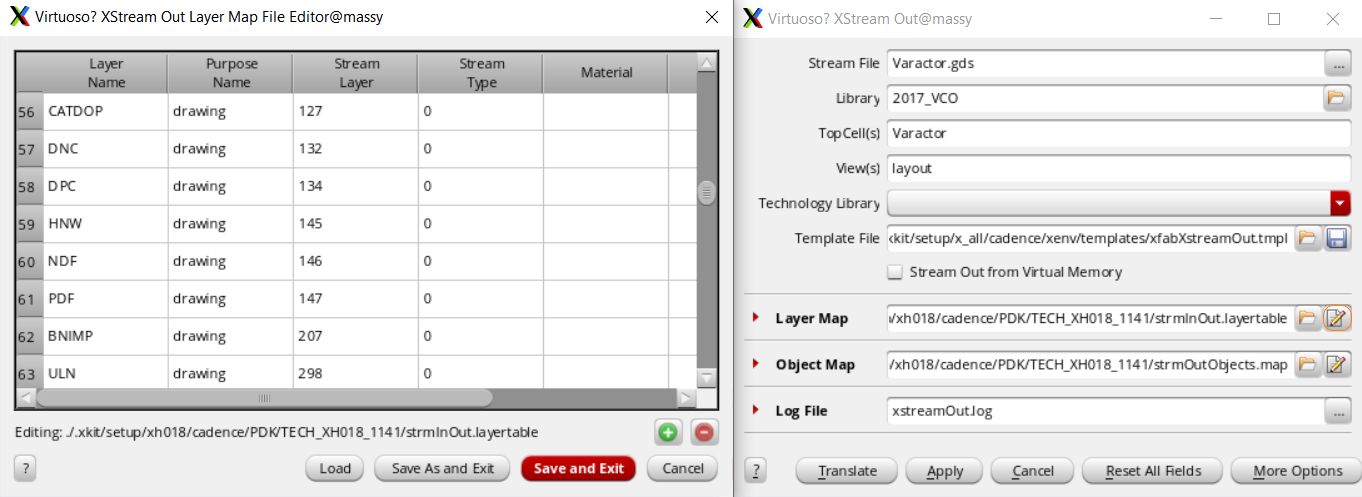
\includegraphics{img/LayerNumbers.png}}
  \subfigure[\label{fig:LayerColors}]{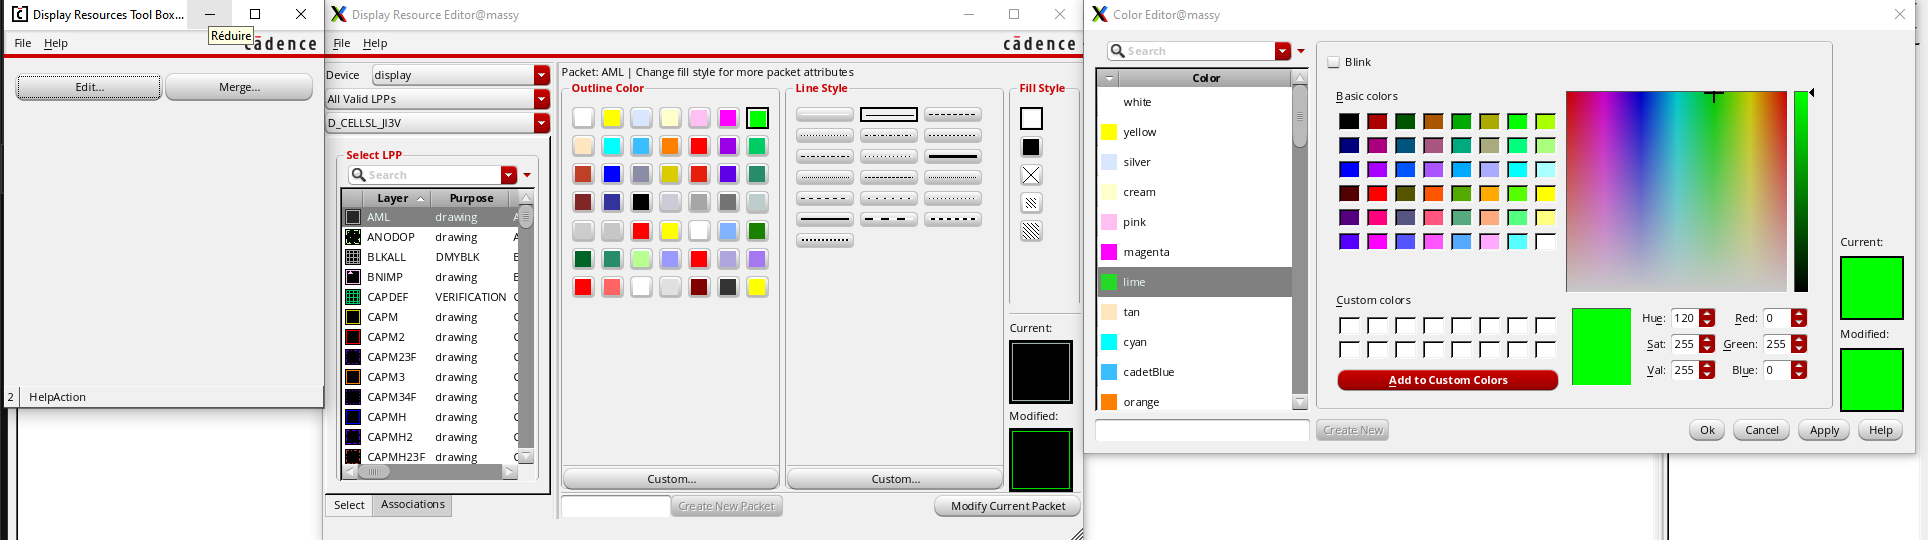
\includegraphics{img/LayerColors.png}}
   \caption{Layer colors map creation using a commercial PDK, where one can verify (a) the layer numbers and (b) the layer colors.}
 \end{center}
\end{figure}

The first scientific paper using he icLayoutRender image rendering tool is from the authors in
 \hyperlink{ref-Martins2021}{(Martins et al., 2021)}, where a voltage-controlled oscillator (VCO) 
is designed. Figure \ref{fig:VCO_color} illustrates such VCO and includes details about the required 
pattern ground shield. Such structure is mandatory for radio frequency circuits, such as a VCO, and 
is only readable if a high quality vectorial image is available. That's the original motivation of the 
authors in proposing icLayoutRender tool. 
\begin{figure}[ht]
\begin{center}
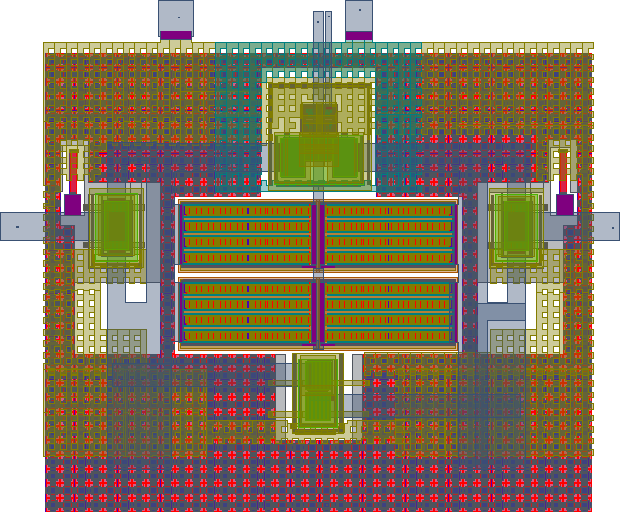
\includegraphics{img/VCO_color.pdf}
\caption{Layout illustration of a VCO from (Martins et al., 2021), including a pattern ground shield.}
\label{fig:VCO_color}
\end{center}\end{figure}

To prove the advantage of using icLayoutRender tool, the authors have
rendered the IC layout known as StrongArm latched comparator and proposed in \hyperlink{ref-Fonseca2017}{(Fonseca et al., 2017)}. 
The original image file is reproduced in Fig \ref{fig:SA_Fonseca} using a gray color scale. Figure \ref{fig:SA_GrayRendering} depicts the
same IC layout rendered by the proposed tool using gray scaled version
of the rendering. A full-color version of this example is depicted in
Fig. \ref{fig:SA_original}. Figure \ref{fig:SA_ColorRendering} IC layout rendered by the proposed tool in full
color map.

\begin{figure}[ht]
 \begin{center}
  \subfigure[\label{fig:SA_Fonseca}]{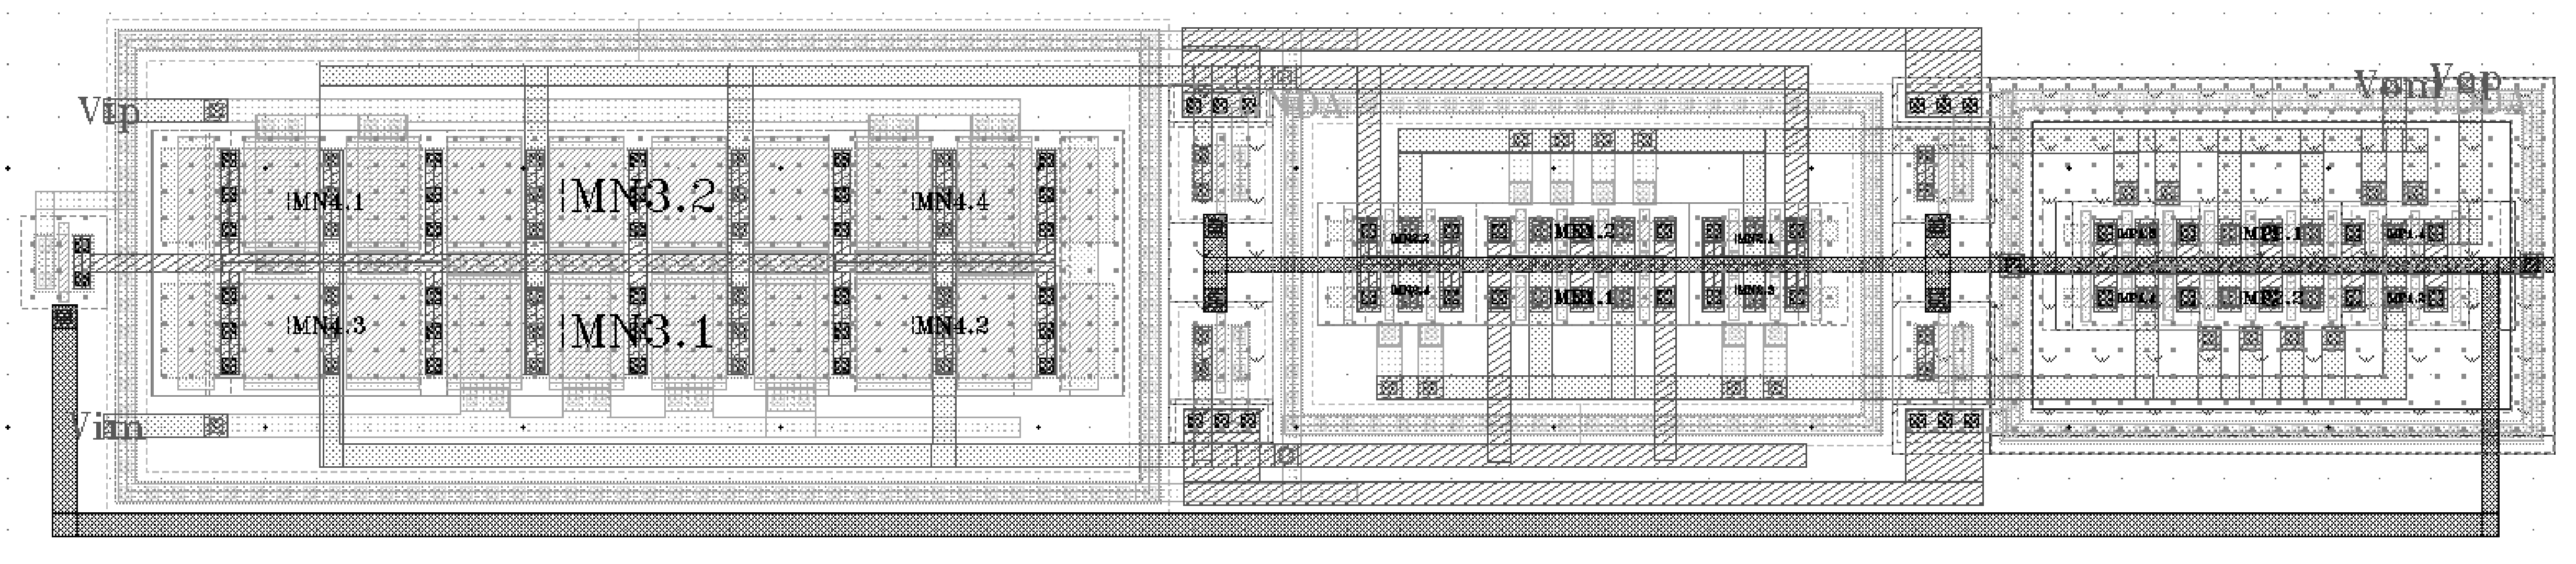
\includegraphics{img/SA_Fonseca.png}}
  \subfigure[\label{fig:SA_GrayRendering}]{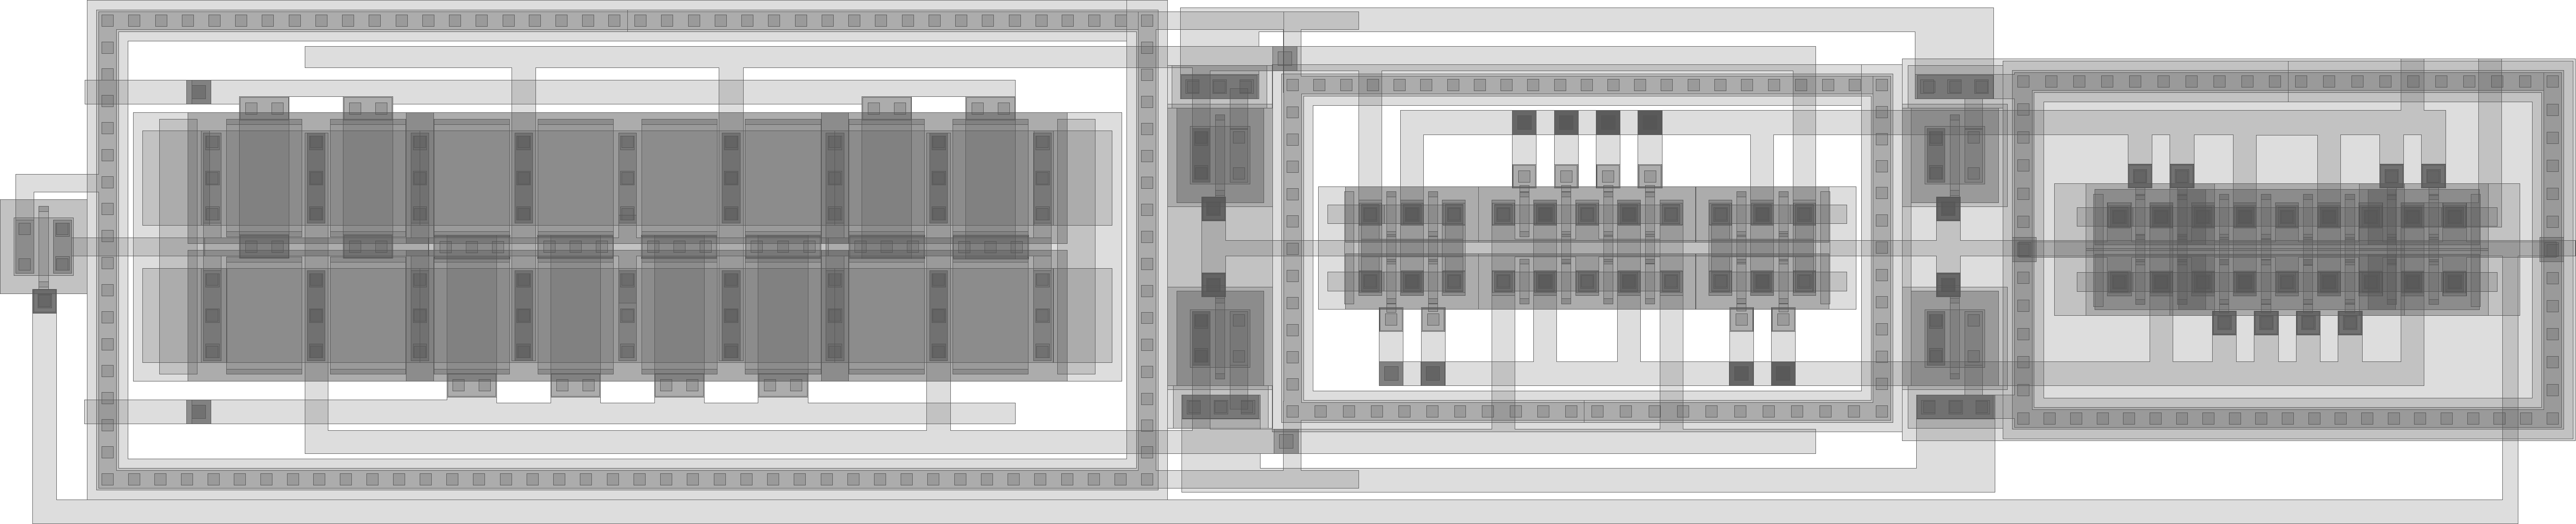
\includegraphics{img/SA_GrayRendering.pdf}}
   \caption{Layout illustration of StrongArm latched comparator proposed in 
   (Fonseca et al., 2017)(a) as its original illustration and (b) using IC layout render tool with gray scale color map.}
 \end{center}
\end{figure}

\begin{figure}[ht]
 \begin{center}
  \subfigure[\label{fig:SA_original}]{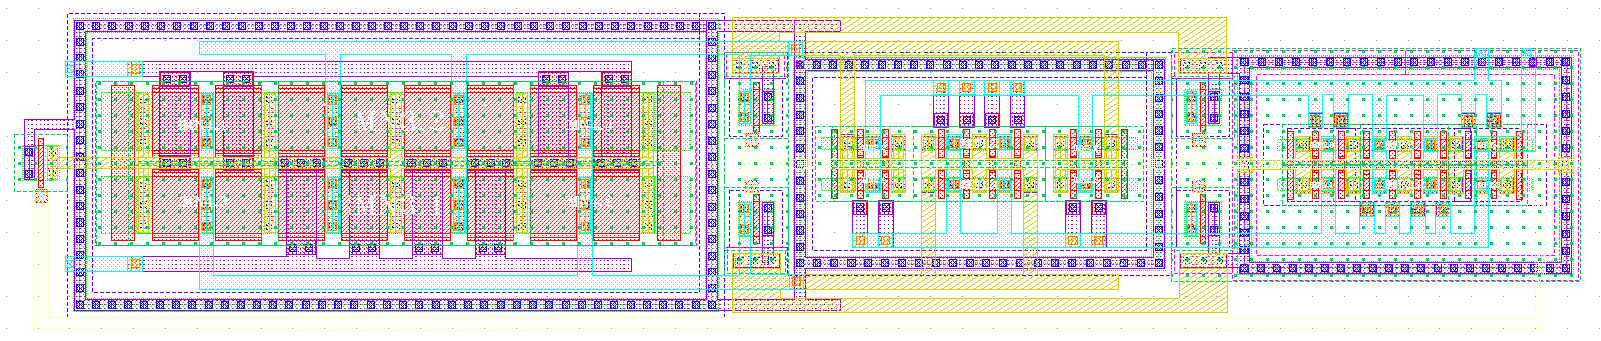
\includegraphics{img/SA_original.png}}
  \subfigure[\label{fig:SA_ColorRendering}]{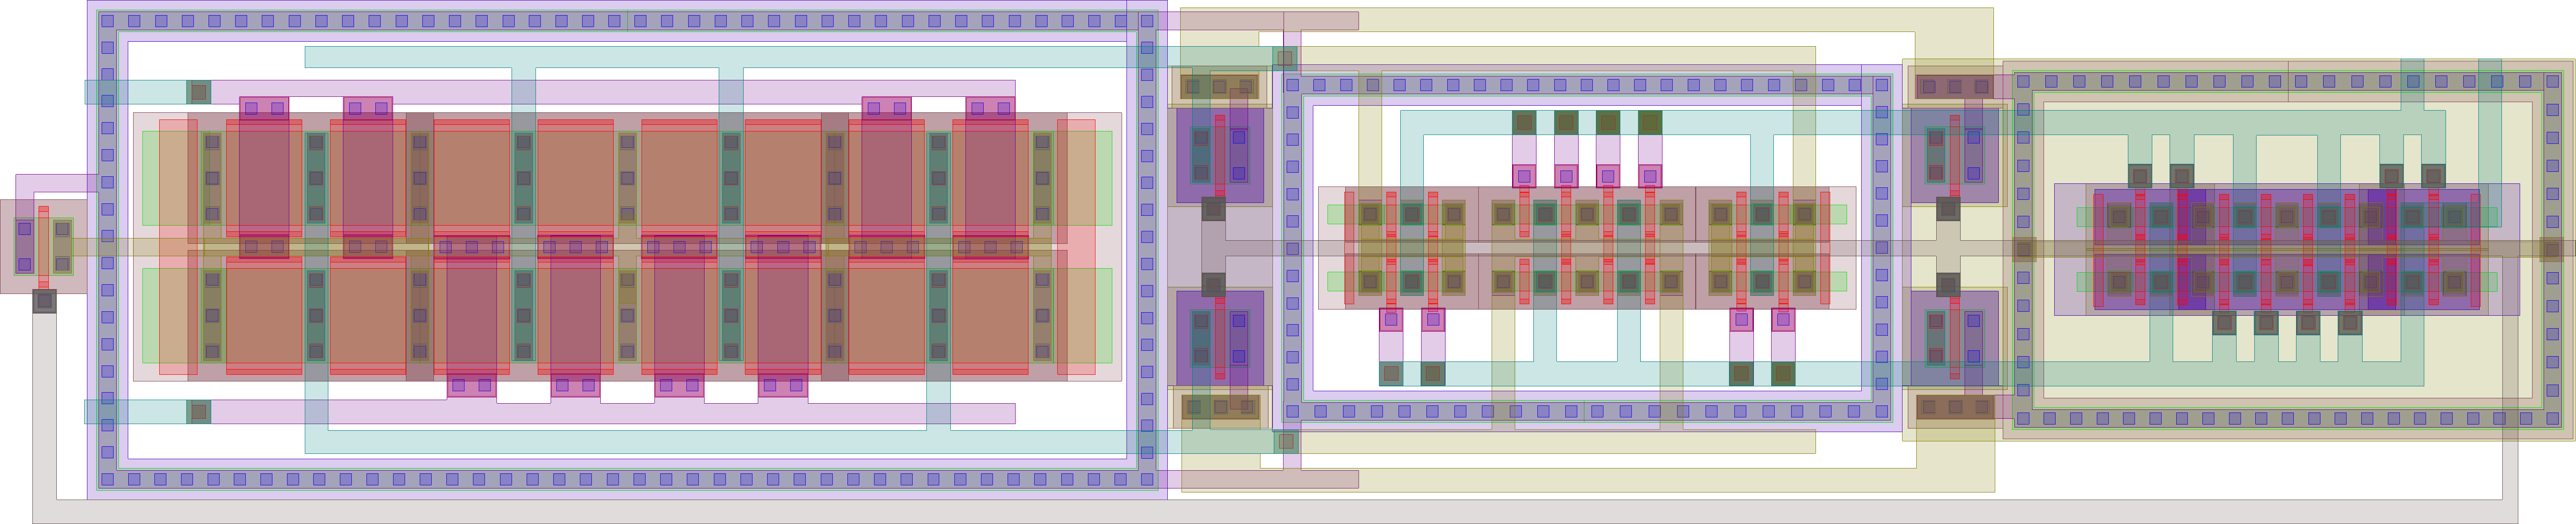
\includegraphics{img/SA_ColorRendering.pdf}}
   \caption{Layout illustration of StrongArm latched comparator proposed in
(Fonseca et al., 2017)(a) in full-color version and (b) using IC
layout render tool with a full-color map.}
 \end{center}
\end{figure}

Another common example depicted in scientific papers is the operational
amplifier. Figure \ref{fig:OTA_original} illustrates an layout example of an amplifier
known as OTA Miler \hyperlink{ref-Ferreira2019b}{(Ferreira et al., 2019)} in its full-color version.
One may observe the readability improvements in Fig. \ref{fig:OTA_ColorRendering}, where IC
Layout Render tool is used.
\begin{figure}[ht]
 \begin{center}
  \subfigure[\label{fig:OTA_original}]{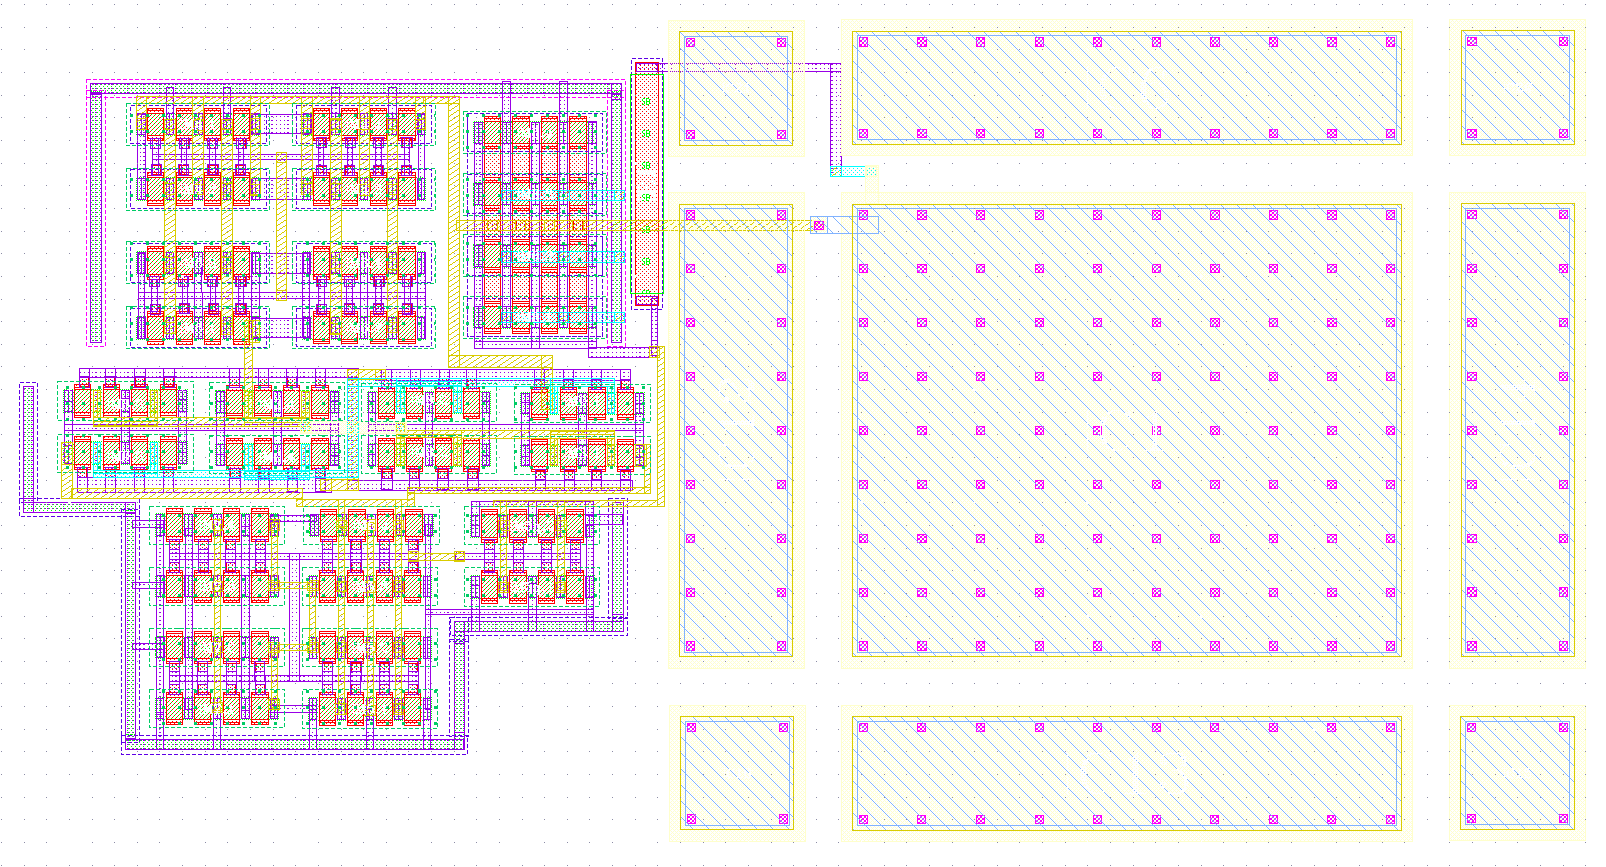
\includegraphics{img/OTA_original.png}}
  \subfigure[\label{fig:OTA_ColorRendering}]{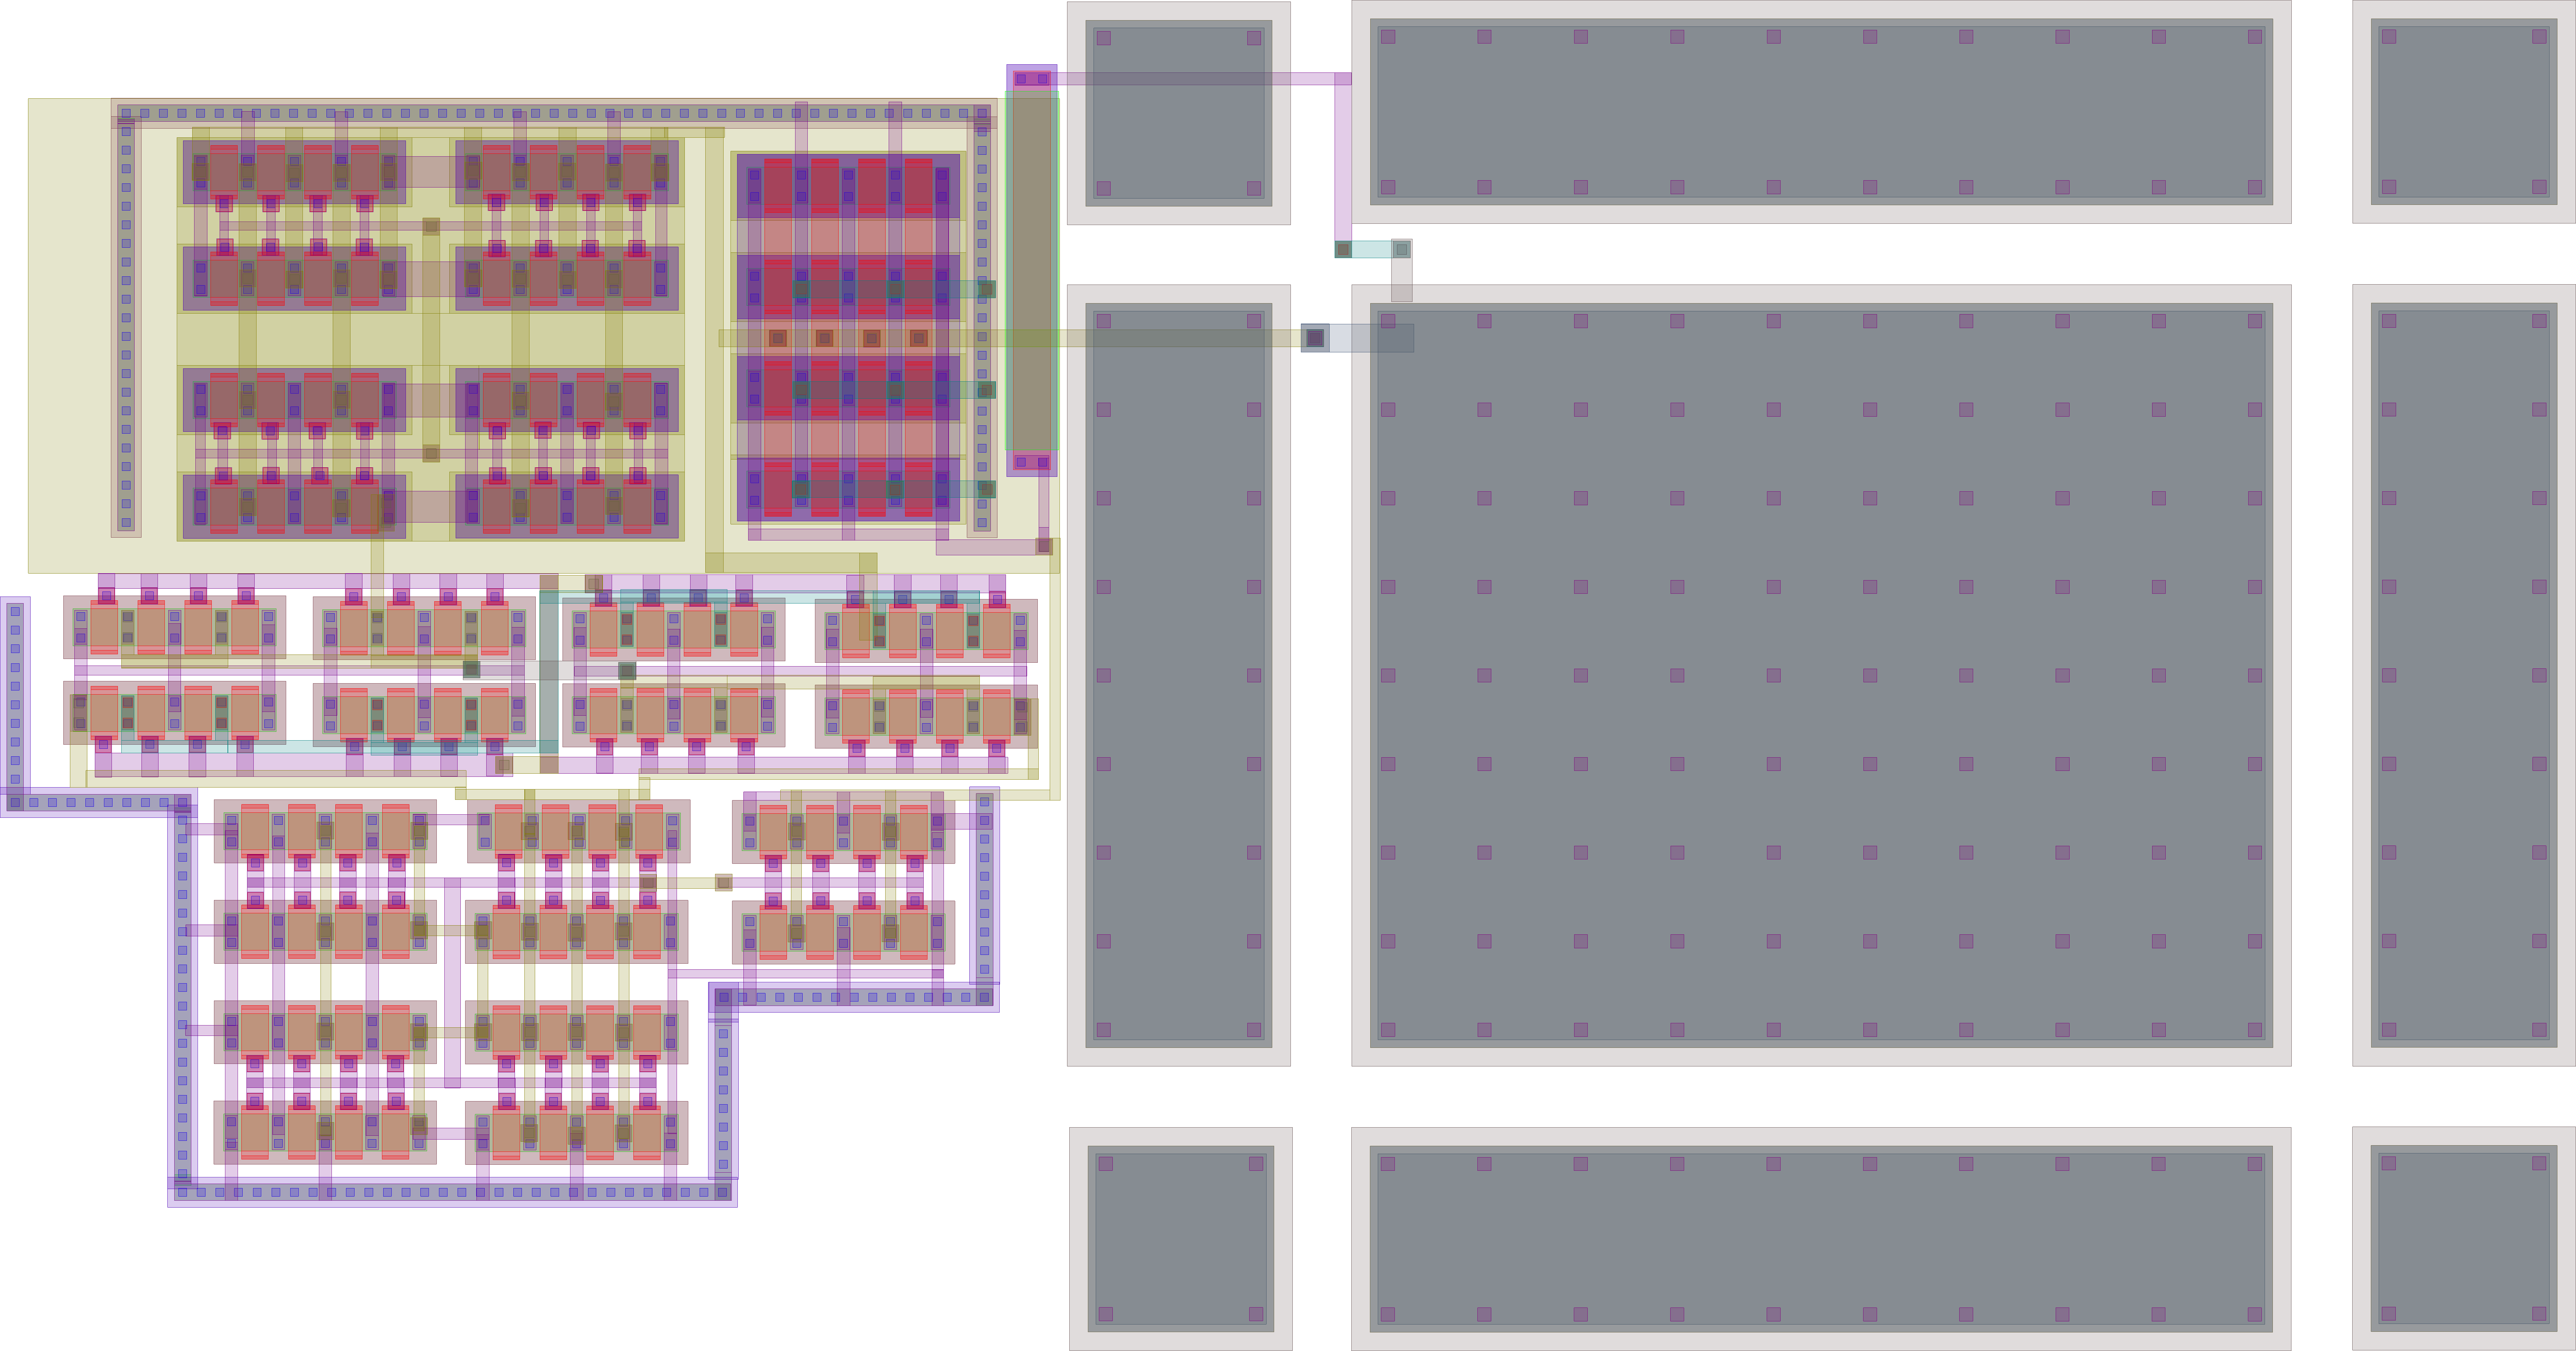
\includegraphics{img/OTA_ColorRendering.pdf}}
   \caption{Layout illustration of original OTA Miler amplifier layout
proposed in (Ferreira et al., 2019) (a) in full-color version and (b)
using IC layout render tool with a full-color map.}
 \end{center}
\end{figure}


\hypertarget{conclusion}{%
\section{Conclusion}\label{conclusion}}

Scientific communications require accurate and repeatable results, where
microelectronics research field requires a high-quality layout
illustration. The proposal demonstrated a user-friendly tool to a GDSII
transcription in a vectorial graph quality image saved as a pdf file.
All illustration examples in this work were obtained from an IC design
using the PDK of \hyperlink{ref-XFAB2019}{(XFAB Mixed-Signal Foundry Experts, 2019)}. However,
layer maps can be easily adapted to any commercial PDK. One may assert
the illustration quality by increasing zoom over Fig. 2, 3 and 4 in the
PDF file or by printing them in a poster-sized version. The vectorial
graphical rendering is obtained by the proposal in which standard tools
are unable to attain.

\hypertarget{references}{%
\section*{References}\label{references}}
\addcontentsline{toc}{section}{References}

\hypertarget{refs}{}
\begin{CSLReferences}{1}{0}
\leavevmode\hypertarget{ref-Calma1987}{}%
Calma Company. (1987). \emph{{GDSII™  Stream Format Manual}} (February).
\url{http://bitsavers.informatik.uni-stuttgart.de/pdf/calma/GDS_II_Stream_Format_Manual_6.0_Feb87.pdf}

\leavevmode\hypertarget{ref-Ferreira2019b}{}%
Ferreira, P. M., Martins, J. R. R. O., Mostafa, A., \& Juillard, J.
(2019). {Process-Voltage-Temperature Analysis of a CMOS-MEMS Readout
Architecture}. \emph{Proc. IEEE Design, Test, Integration \& Packaging
of MEMS/MOEMS}, 1--4. \url{https://doi.org/10.1109/DTIP.2019.8752699}

\leavevmode\hypertarget{ref-Fonseca2017}{}%
Fonseca, A. V., Khattabi, R. E., Afshari, W. A., Barúqui, F. A. P.,
Soares, C. F. T., \& Ferreira, P. M. (2017). {A Temperature-Aware
Analysis of Latched Comparators for Smart Vehicle Applications}.
\emph{Proc ACM IEEE Symp. Integr. Circuits Syst. Design}, 1--6.
\url{https://doi.org/10.29292/jics.v13i1.8}

\leavevmode\hypertarget{ref-Martins2021}{}%
Martins, J. R. O. R., Alves, F., \& Ferreira, P. M. (2021). {A 237 ppm /
°C L-Band Active Inductance Based Voltage Controlled Oscillator in SOI
0.18 µm}. \emph{Proc ACM IEEE Symp. Integr. Circuits Syst. Design},
1--6. \url{https://doi.org/10.1109/SBCCI53441.2021.9529990}

\leavevmode\hypertarget{ref-Vollmer2020}{}%
Vollmer, R. (2020). \emph{{GDSLatexConverter}}.
\url{https://github.com/Aypac/GDSLatexConverter}

\leavevmode\hypertarget{ref-XFAB2019}{}%
XFAB Mixed-Signal Foundry Experts. (2019). \emph{{XH018 - 0.18 Micron
Modular Analog Mixed HV Technology}} (pp. 1--22).
\url{https://www.xfab.com/technology/cmos/018-um-xh018/}

\end{CSLReferences}

\end{document}

